\documentclass[12pt,AutoFakeBold]{article} 

\usepackage[数字信号处理]{XDUreport}  % 科目名称
\problem{数字信号处理设计与仿真分析}  % 请在此处填写问题内容
% 其他参数在宏包中进行更改,其中学院,班级,姓名,学号均在sty宏包内进行更改
% \usepackage{fourier}  % 这是 fourier 字体,更柔和 

%% 如果你需要中文的一级标题编号,如“一、”、“二、”等,请把下面两行取消注释
% \RequirePackage{zhnumber} % change section number to chinese
% \titleformat{\section}{\Large\bfseries\rmfamily}{\zhnum{section}、}{0em}{}

% 文档开始
        
\begin{document}

\maketitle
\setcounter{tocdepth}{2}

\tableofcontents  % 生成目录

% 正文标题
\makeatletter
\begin{center}
    \LARGE \textbf{\textsf{\@problem}}
\end{center}
\makeatother

% 正文开始

\section{问题描述}

\begin{enumerate}[(1)]
\item 建立两个模拟信号的数学模型 $sa_1(t)$ 和 $sa_2(t)$,其中 $sa_1(t)$ 是有用信号,$sa_2(t)$ 是干扰信号。两个信号的中心频率、信号带宽等参数由学生自己选定,要求两个信号的频谱不重叠,$sa_2(t)$ 的幅度比 $sa_1(t)$ 的幅度高 $20\mathrm{dB}$,两个信号时域叠加得到合成信号 $xa(t)$,即
%
\begin{equation*}
xa(t)=sa_1(t)+sa_2(t)
\end{equation*}
%
设计计算机程序仿真产生 $sa_1(t)$、$sa_2(t)$、$xa(t)$ 信号,分别画出三个模拟信号的时域波形和频谱图;

\item 根据 $xa(t)$ 的中心频率和带宽,按照奈奎斯特采样定理选择采样频率 $f_s$,分别对信号 $sa_1(t)$、$sa_2(t)$、$xa(t)$ 进行时域采样,得到离散信号 $s_1(n)$、$s_2(n)$、$x(n)$。利用 FFT 算法分析离散信号的频谱,分别画出三个离散信号的时域波形和频谱图;

\item 设计数字滤波器 $H(z)$,要求该滤波器对干扰信号 $s_2(n)$ 的衰减大于 $40\mathrm{dB}$。提出滤波器的设计指标,并设计滤波器,给出滤波器的设计结果,绘制滤波器的幅频特性和相频特性曲线,验证滤波器的设计结果是否达到设计指标要求;

\item 选择实现数字滤波器 $H(z)$ 的结构,画出结构信号流图;

\item 将合成信号 $x(n)$ 输入数字滤波器 $H(z)$,按照所选择的滤波器结构,设计计算机程序计算滤波器的输出响应 $y(n)$,画出 $y(n)$ 的时域波形和频谱图;

\item 分析、总结设计结果,提交课程设计报告。
\end{enumerate}

\section{实验环境}

\begin{itemize}
\item Matlab: 编写代码并编译运行。
\item JupyterNotebook: 编写 Python 代码并生成 notebook 的 pdf 文件添加在附录中。
\item \LaTeX: 进行文档编写和排版。
\item Visio: 绘制流程图和信号流图。
\end{itemize}

\section{基础知识回顾}

\subsection{参数概念}

\begin{enumerate}[1.]
\item 中心频率 (Center frequency): 周期信号对应的频率,可以通过傅里叶级数转换为不同频率弦波的和。
\item 信号带宽 (Bandwidth): 信号所占据的频带宽度;在被用来描述信道时,带宽是指能够有效通过该信道的信号的最大频带宽度。对于模拟信号而言,带宽又称为频宽,以赫兹(Hz)为单位。对于数字信号而言,带宽是指单位时间内链路能够通过的数据量。
\end{enumerate}

\subsection{奈奎斯特采样定理}

一个有带限的连续时间信号可以被采样并从它的样本中完美恢复,如果波形的采样频率是它的最高频率分量的两倍以上。(A bandlimited continuous-time signal can be sampled and perfectly reconstructed from its samples if the waveform is sampled over twice as fast as it's highest frequency component)

\subsection{数字滤波器}

数字滤波器是对数字信号进行滤波处理以得到期望的响应特性的离散时间系统。作为一种电子滤波器,数字滤波器与完全工作在模拟信号域的模拟滤波器不同。数字滤波器工作在数字信号域,它处理的对象是经由采样器件将模拟信号转换而得到的数字信号。线性非时变的数字滤波器包括无限长脉冲响应滤波器(IIR滤波器)和有限长脉冲响应滤波器(FIR滤波器)两种。这两种滤波器的系统函数可以统一以 Z 变换表示为:
%
\begin{equation}
H(z)=\frac{B(z)}{A(z)}=\frac{b_0+b_1z^{-1}+b_2z^{-2}+\cdots+b_Nz^{-N}}{1+a_1z^{-1}+a_2z^{-2}+\cdots+a_Mz^{-M}}
\end{equation}
%
当 $M\ge1$ 时,$M$ 就是 IIR 滤波器的阶数,表示系统中反馈环的个数。由于反馈的存在,IIR 滤波器的脉冲响应为无限长,因此得名。若 $A(z)=1$,则系统的脉冲响应的长度为 $N+1$,故而被称作 FIR 滤波器。

\subsection{信号流图}

信号流图示一种表示一组联立线形代数方程的图。表明了系统中各信号的关系,包含了结构图中所包含的全部信息,与结构图一一对应。

\section{方案设计}

按如图 \ref{fig:workflow} 所示的实验流程图进行问题求解。用 Matlab 和 Python 两种语言编写代码实现,正文中的实验图为 Matlab 运行结果,Python 运行结果与 Matlab 相似,为避免赘述放在附录以供检验对比。

\begin{figure}[htbp]
	\centering
	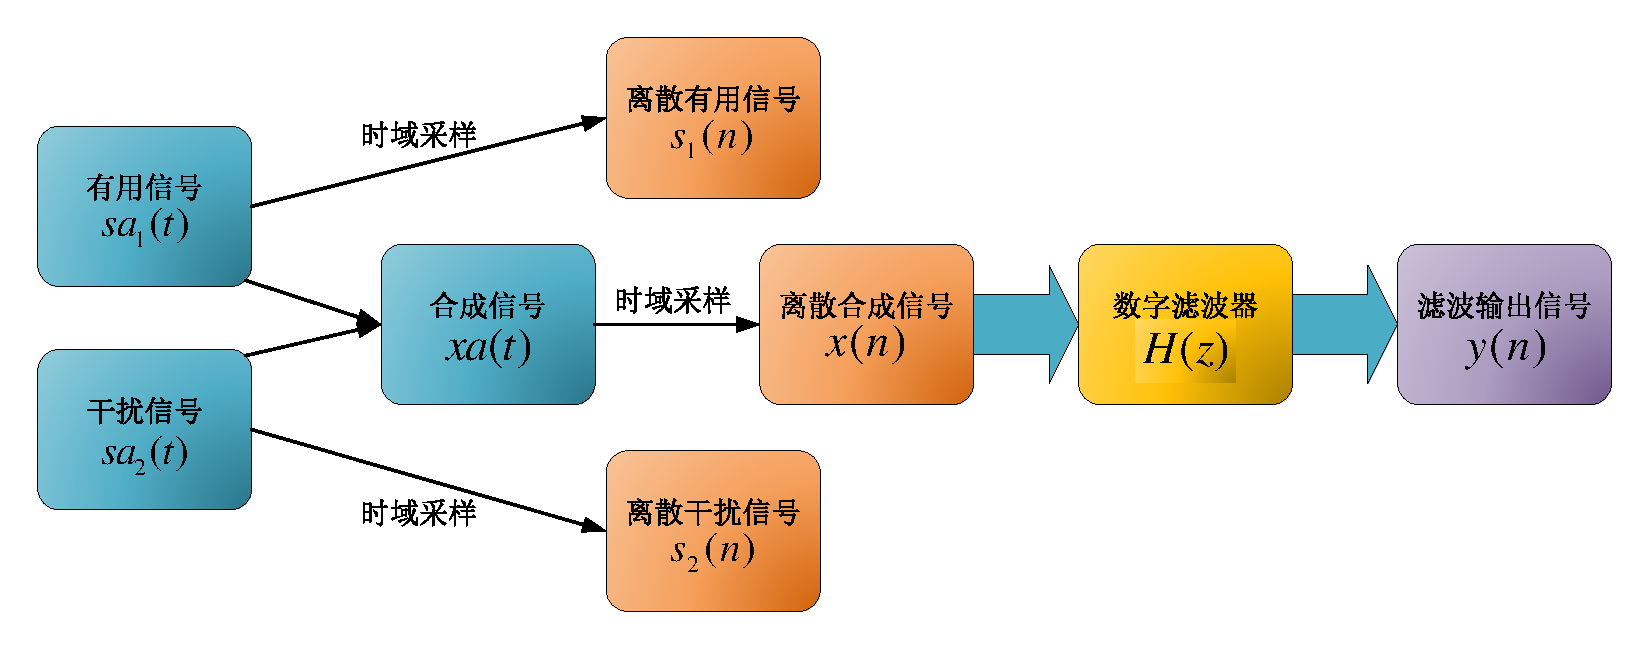
\includegraphics[width=\textwidth]{figure/workflow.pdf}
	\caption{实验流程图} \label{fig:workflow}
\end{figure}

\section{问题求解}

\subsection{问题 1}

假设有用信号为 $sa_1(t)=\cos(2\pi f_1t)+\cos(2\pi f_2t)$,其中 $f_1=10Hz, f_2=6Hz$,则周期 $T_1=0.5s$。作傅里叶变换得 
%
\begin{align}
F_1(j2\pi f) &= \pi\left[\delta(2\pi(f+f_1))+\delta(2\pi(f-f_1))+\delta(2\pi(f+f_2))+\delta(2\pi(f-f_2))\right] \\
 &= \frac{1}{2}\left[\delta(f+10)+\delta(f-10)+\delta(f+6)+\delta(f-6)\right] 
\end{align}
%
有用信号 $sa_1(t)$ 时域波形和频谱图如图 \ref{fig:sa1} 所示。

\begin{figure}[htbp]
	\centering
	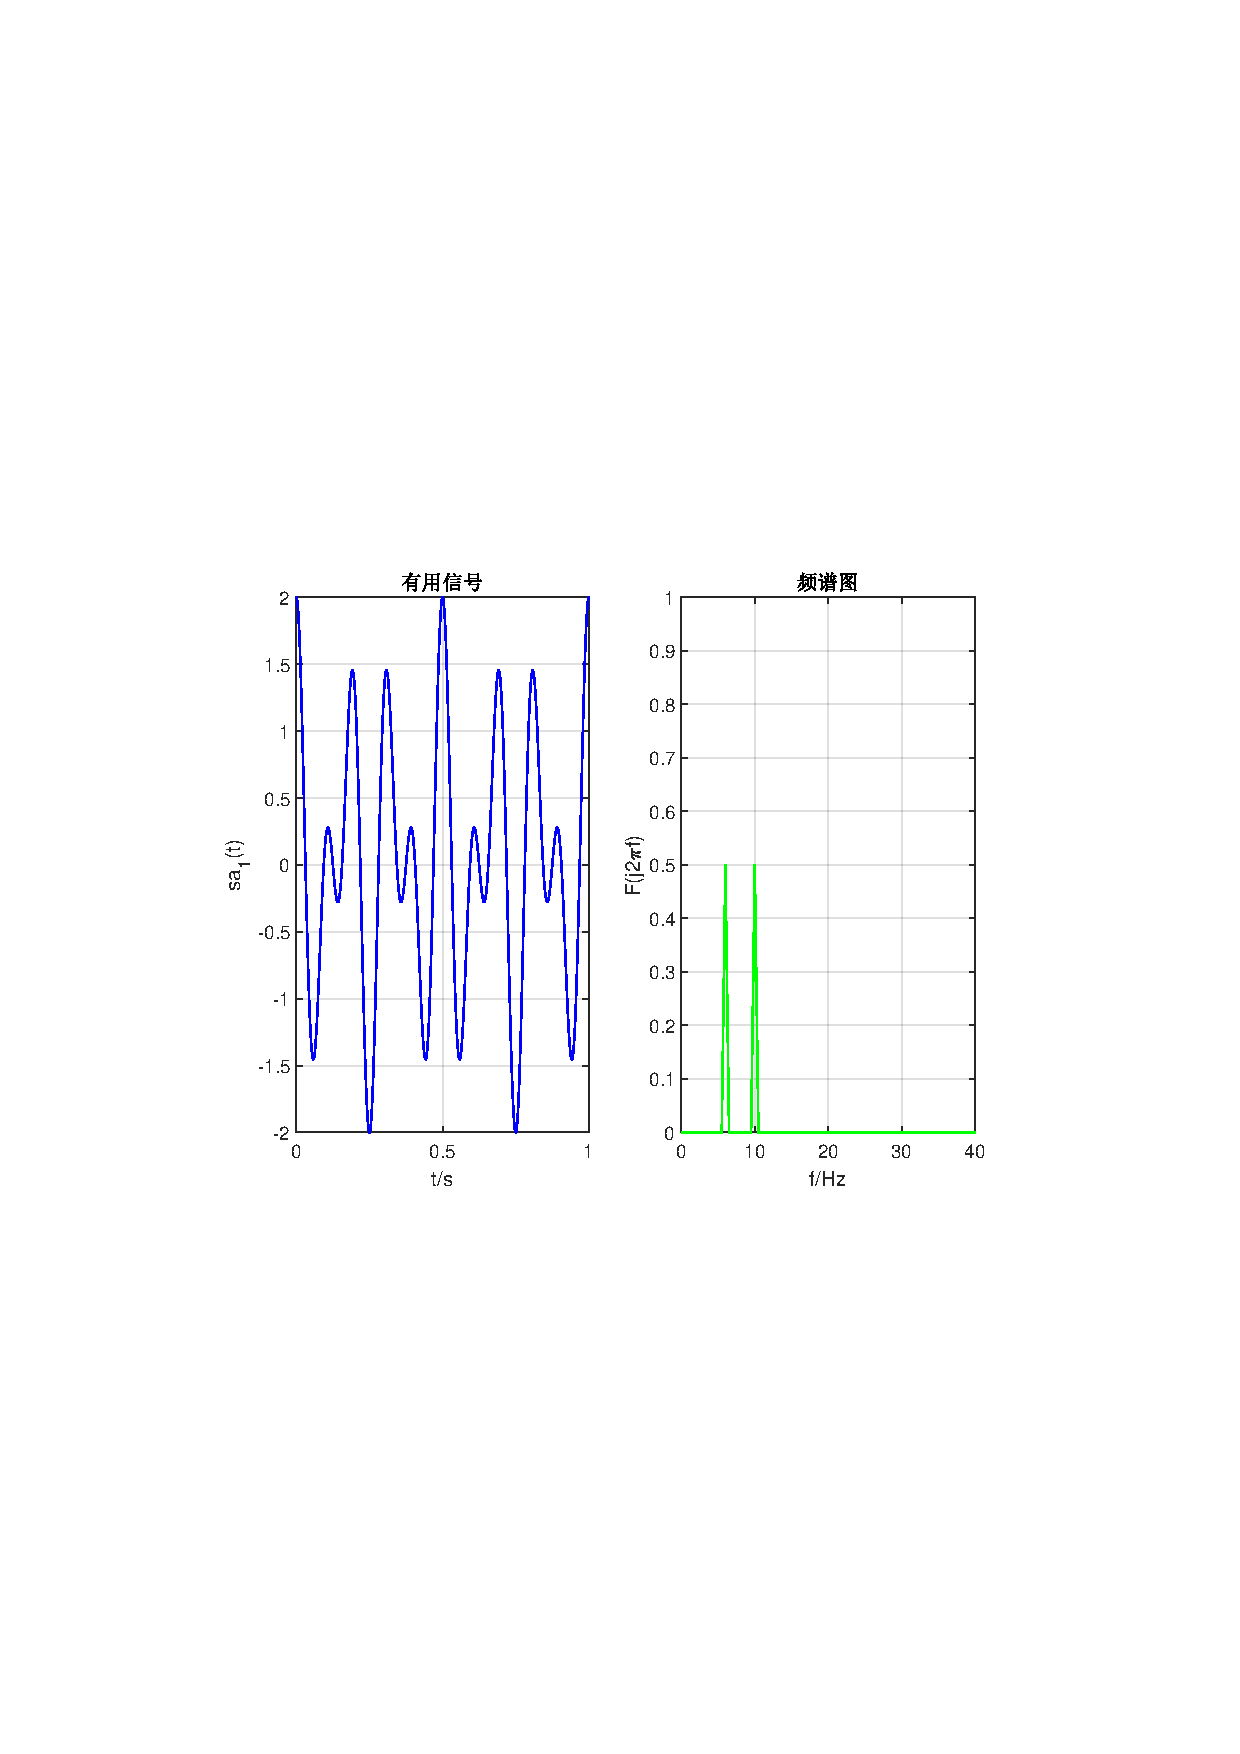
\includegraphics[width=0.7\textwidth]{figure/sa1.pdf}
	\caption{有用信号 $sa_1(t)$ 时域波形和频谱图} \label{fig:sa1}
\end{figure}

假设干扰信号 $sa_2(t)$ 的幅度是 $sa_1(t)$ 的 $x$ 倍,$sa_1(t)$ 幅度比 $sa_2(t)$ 高 $20\mathrm{dB}$,则 $20\lg{x}=20$,解得 $x=10$。可假设干扰信号为 $sa_2(t)=10\cos(2\pi f_3t)+10\cos(2\pi f_4t)$,其中 $f_3=36Hz, f_4=25Hz$,则周期 $T_2=1s$。作傅里叶变换得 
%
\begin{align}
F_2(j2\pi f) &= 10\pi\left[\delta(2\pi(f+f_3))+\delta(2\pi(f-f_3))+\delta(2\pi(f+f_4))+\delta(2\pi(f-f_4))\right] \\
 &= 5\left[\delta(f+36)+\delta(f-36)+\delta(f+25)+\delta(f-25)\right]
\end{align}
%
干扰信号 $sa_2(t)$ 时域波形和频谱图如图 \ref{fig:sa2} 所示。

\begin{figure}[htbp]
	\centering
	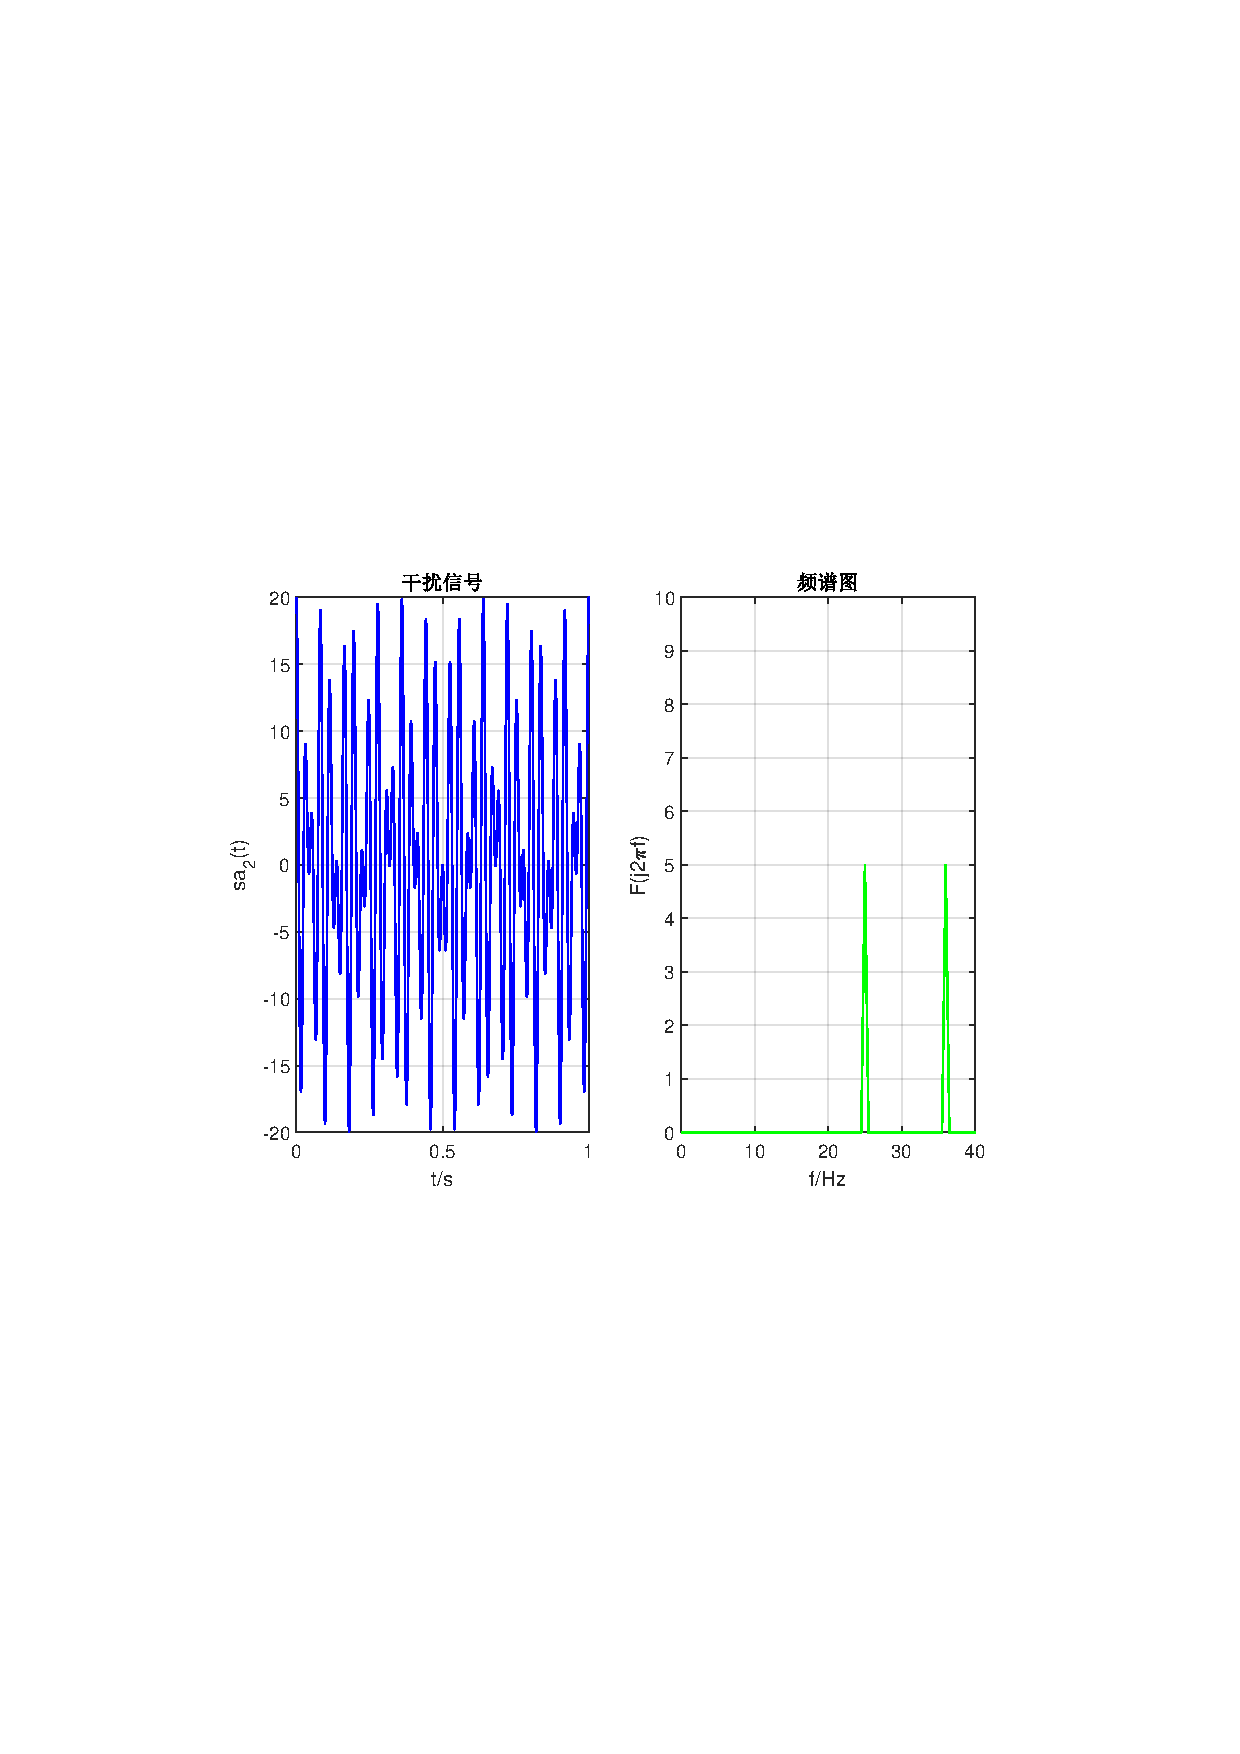
\includegraphics[width=0.7\textwidth]{figure/sa2.pdf}
	\caption{干扰信号 $sa_2(t)$ 时域波形和频谱图} \label{fig:sa2}
\end{figure}

两个信号时域叠加得到合成信号
%
\begin{equation}
xa(t)=sa_1(t)+sa_2(t)=\cos(2\pi f_1t)+\cos(2\pi f_2t)+10\cos(2\pi f_3t)+10\cos(2\pi f_4t)
\end{equation}
%
其周期 $T_3=1s$。合成信号 $xa(t)$ 时域波形和频谱图如图 \ref{fig:xa} 所示。

\begin{figure}[htbp]
	\centering
	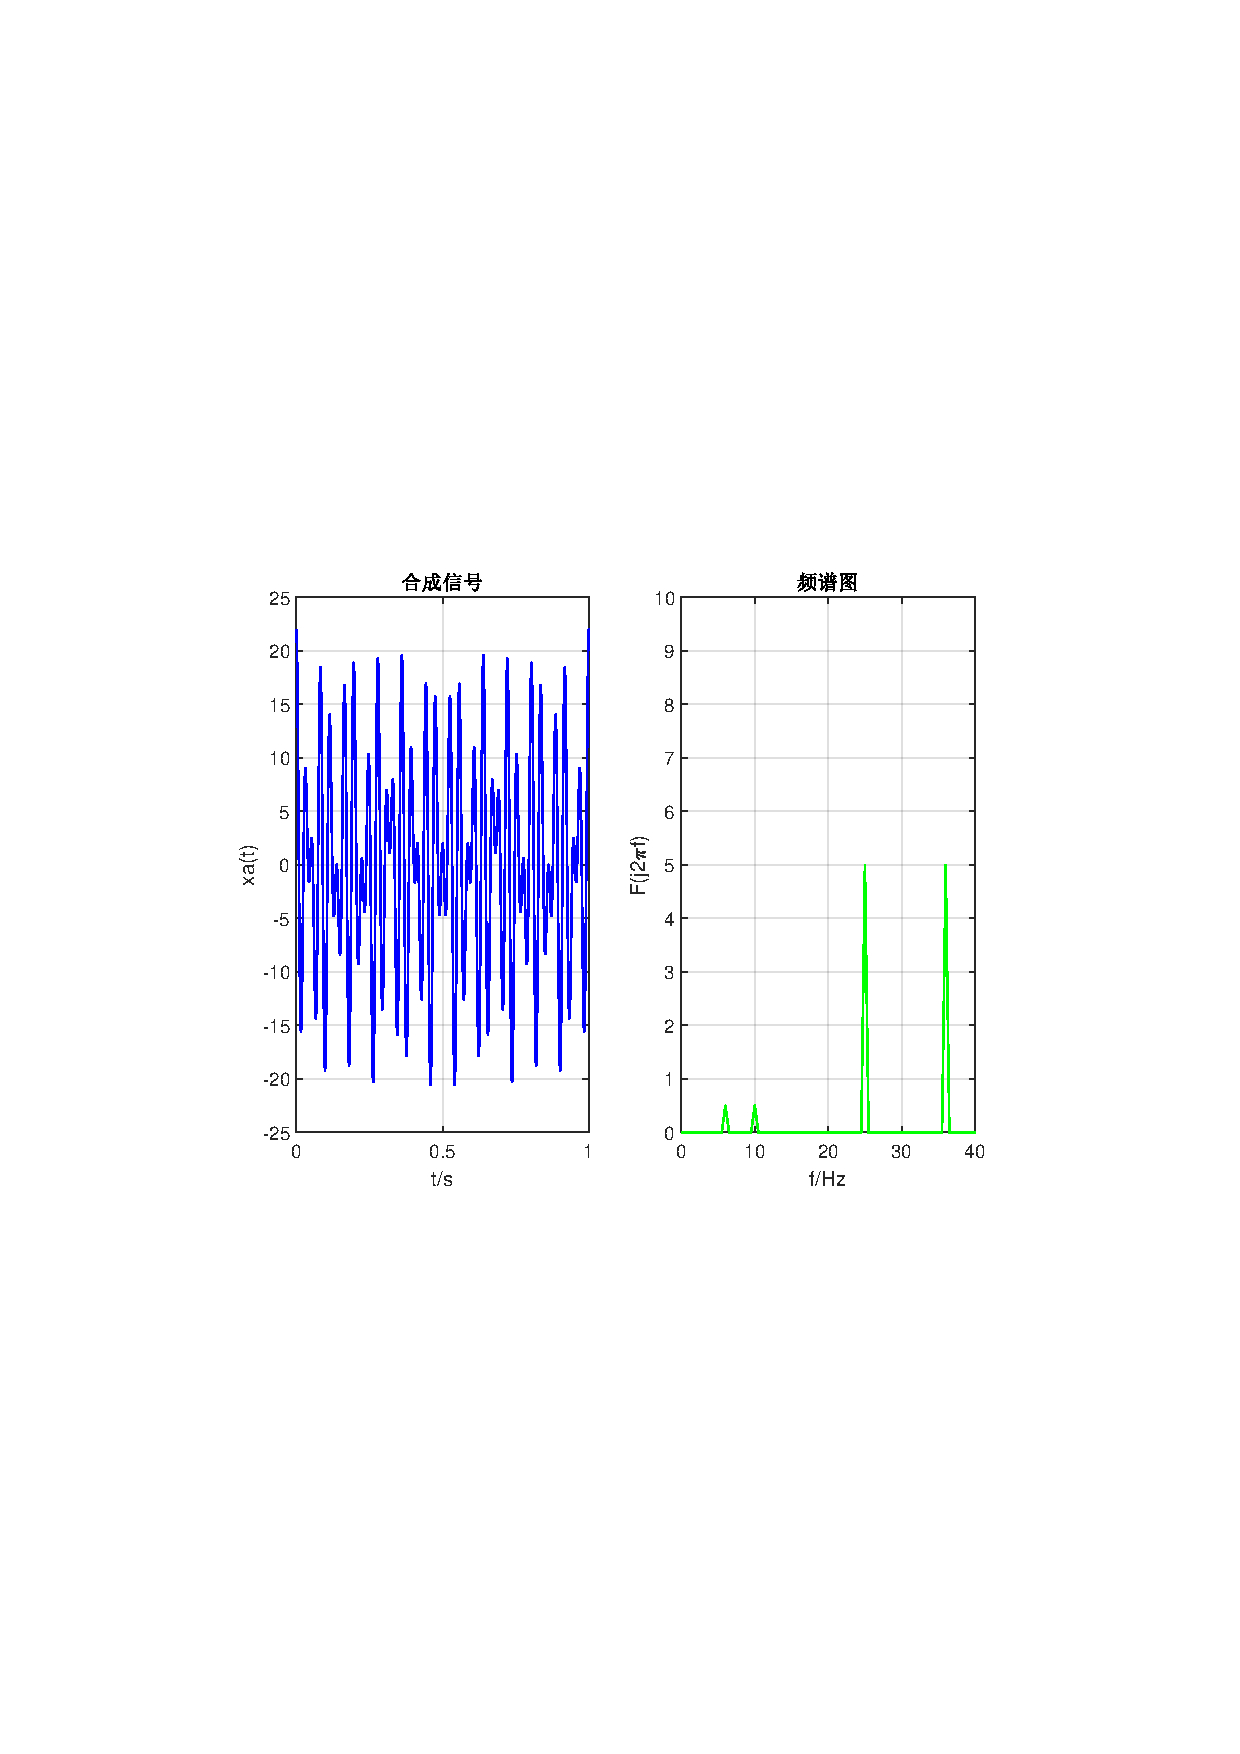
\includegraphics[width=0.7\textwidth]{figure/xa.pdf}
	\caption{合成信号 $xa(t)$ 时域波形和频谱图} \label{fig:xa}
\end{figure}

\subsection{问题 2}

$x_a(t)$ 的最高频率 $f_{c}=36Hz$,那么奈奎斯特采样频率 $f_{s}=2f_{c}=72Hz$,选择采样频率 $100Hz$ 进行采样。

对信号 $sa_1(t)$ 进行采样,并作 200 点 FFT,得到离散有用信号 $s_1(n)$ 的时域波形和频谱图如图 \ref{fig:sn1} 所示。 

\begin{figure}[htbp]
	\centering
	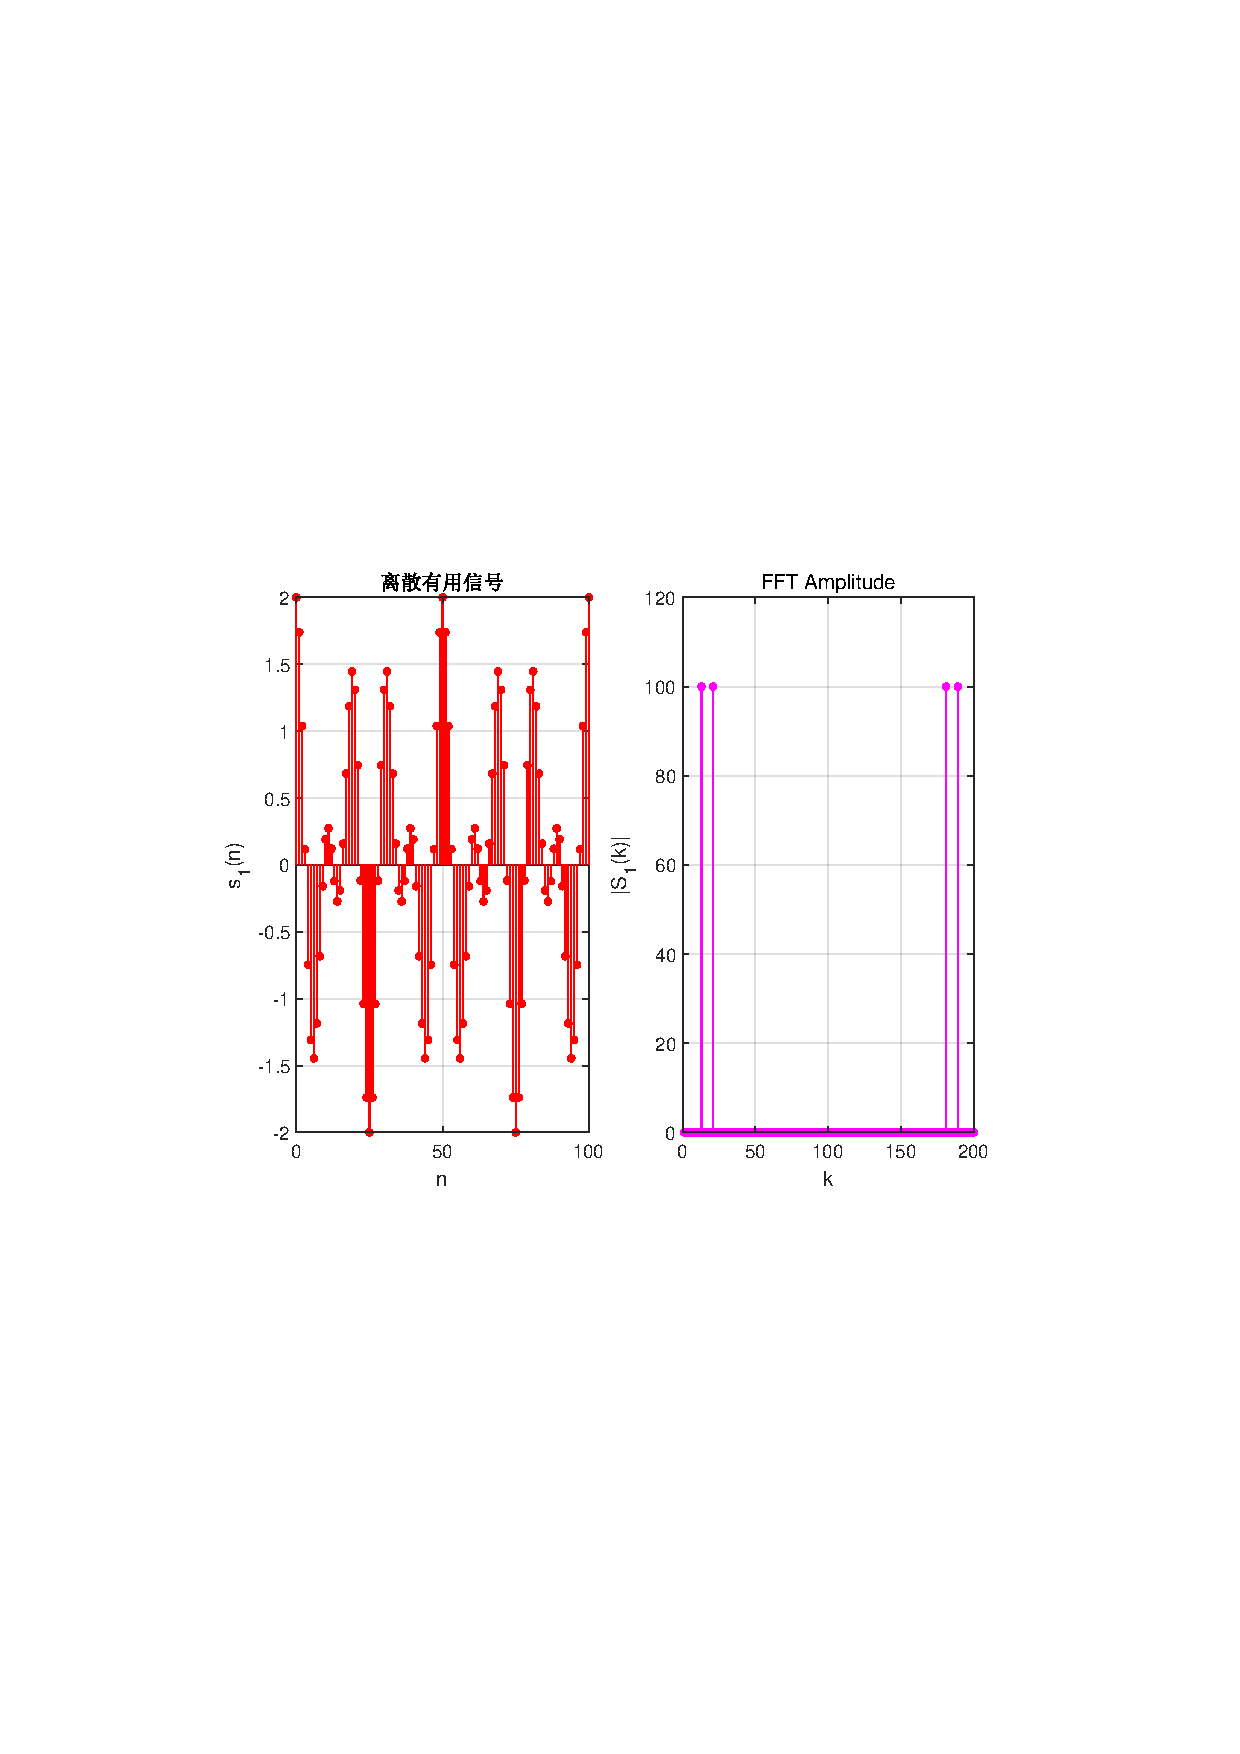
\includegraphics[width=0.7\textwidth]{figure/sn1.pdf}
	\caption{离散有用信号 $s_1(n)$ 的时域波形和频谱图} \label{fig:sn1}
\end{figure}

对信号 $sa_2(t)$ 进行采样,并作 200 点 FFT,得到离散干扰信号 $s_2(n)$ 的时域波形和频谱图如图 \ref{fig:sn2} 所示。 

\begin{figure}[htbp]
	\centering
	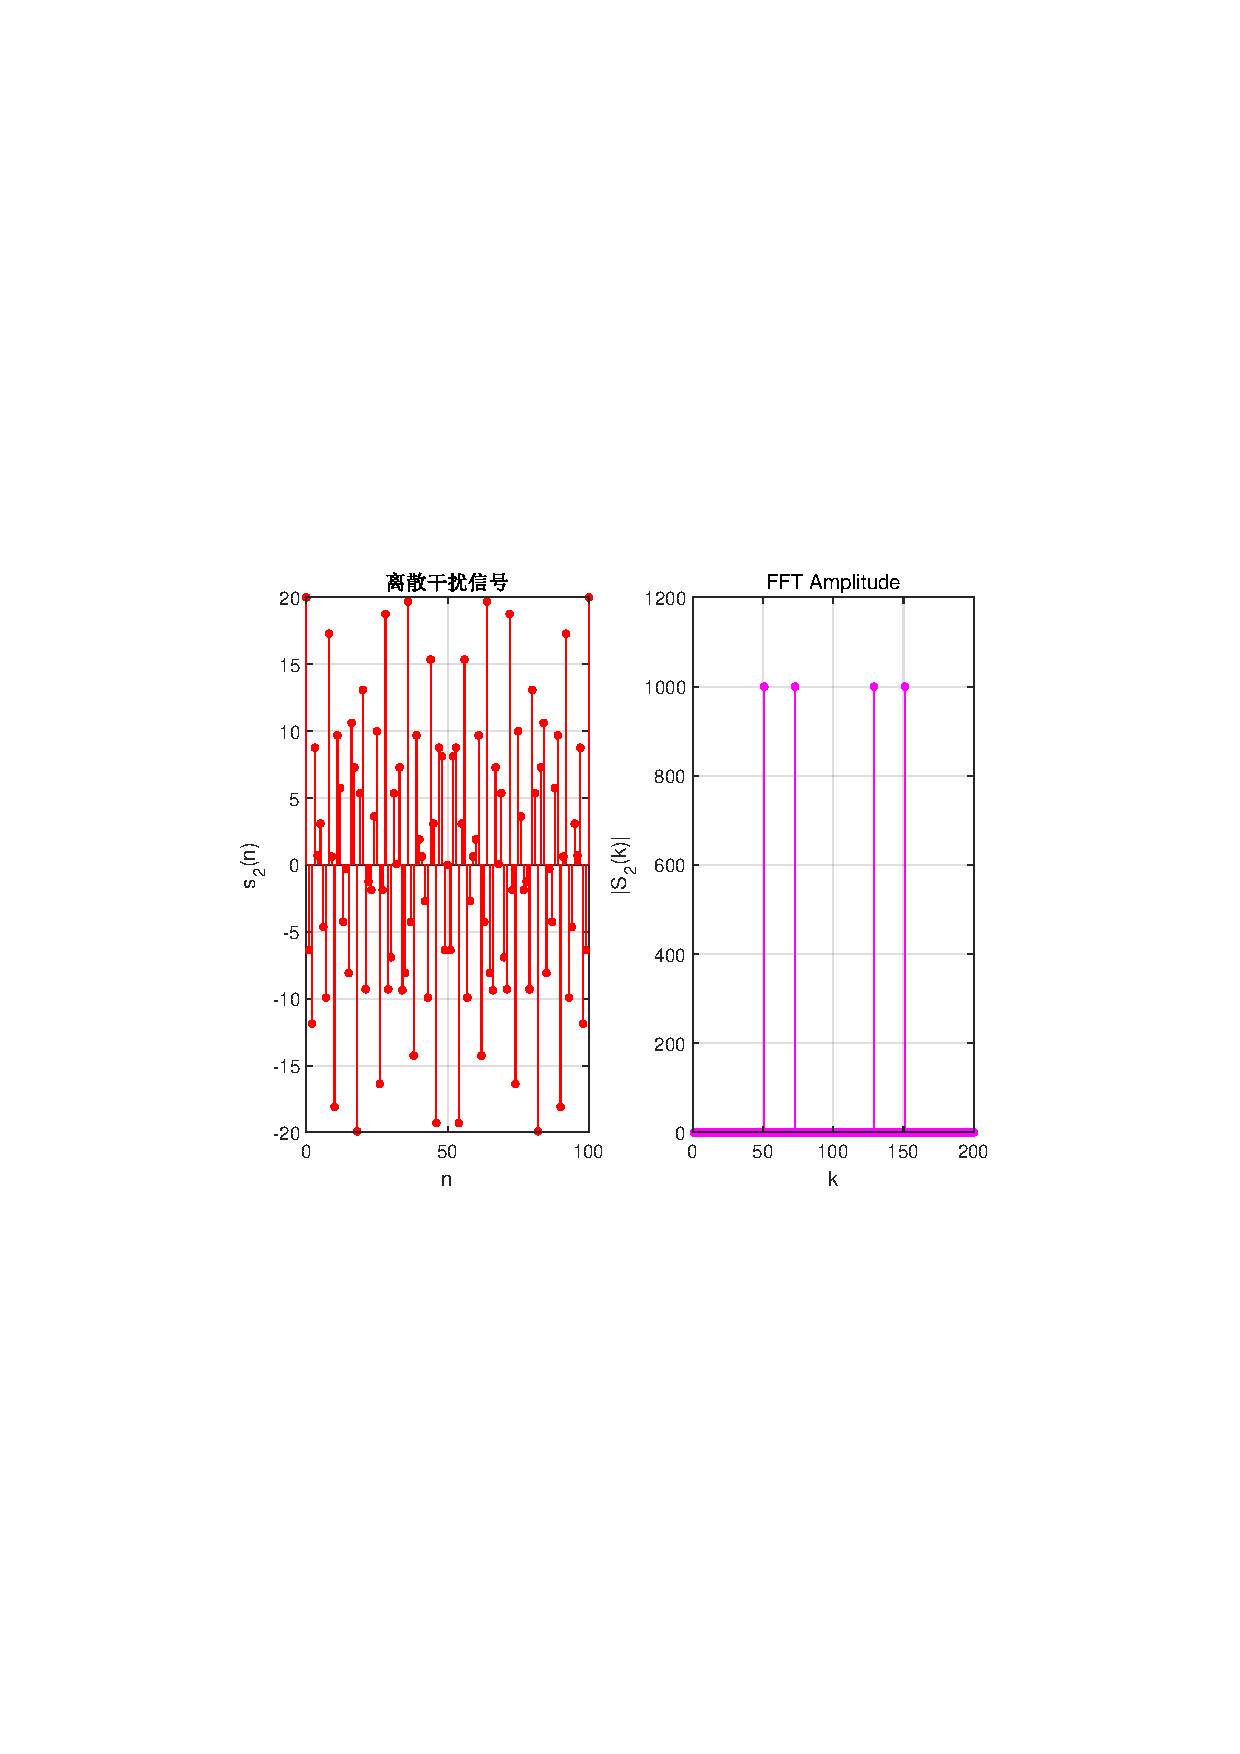
\includegraphics[width=0.7\textwidth]{figure/sn2.pdf}
	\caption{离散干扰信号 $s_2(n)$ 的时域波形和频谱图} \label{fig:sn2}
\end{figure}

对信号 $xa(t)$ 进行采样,并作 200 点 FFT,得到离散合成信号 $x(n)$ 的时域波形和频谱图如图 \ref{fig:xn} 所示。 

\begin{figure}[htbp]
	\centering
	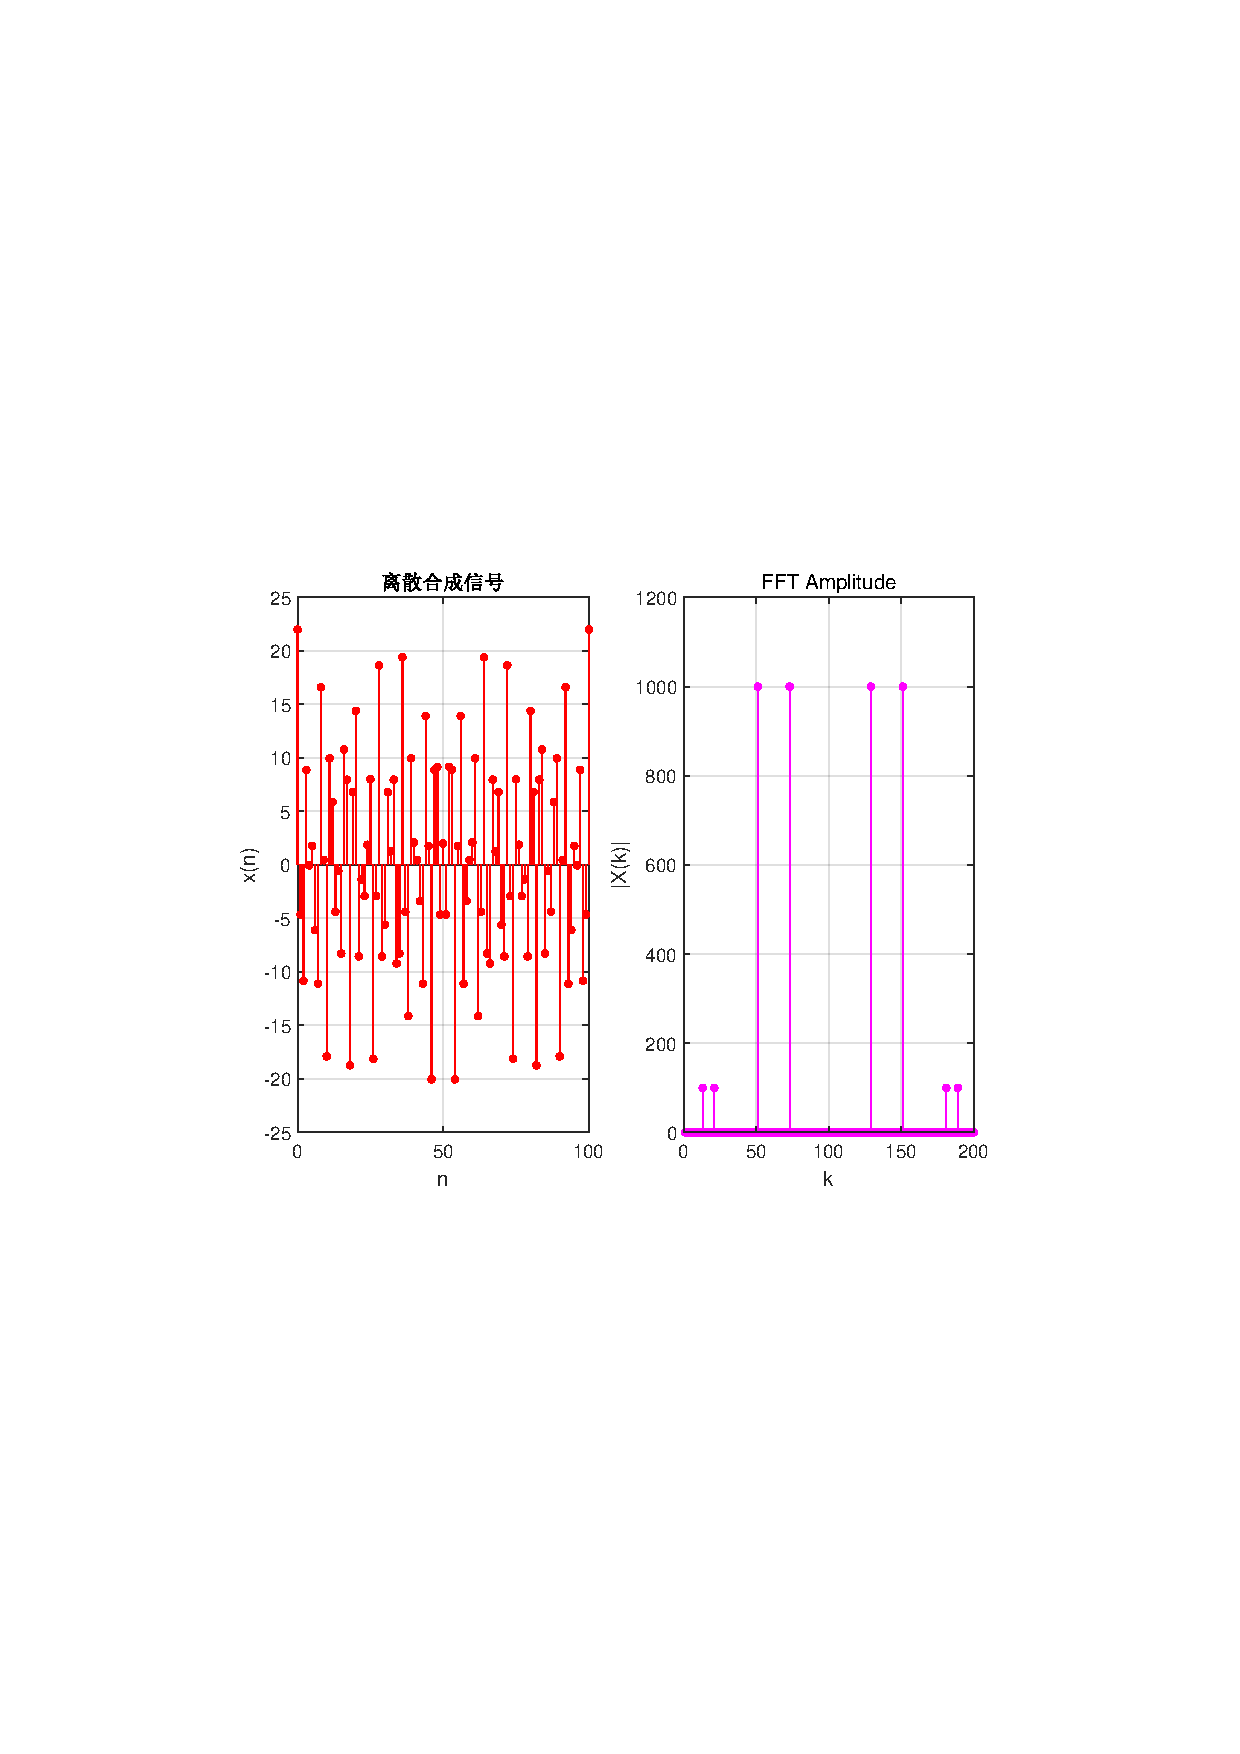
\includegraphics[width=0.7\textwidth]{figure/xn.pdf}
	\caption{离散合成信号 $x(n)$ 的时域波形和频谱图} \label{fig:xn}
\end{figure}

\subsection{问题 3}

采用数字巴特沃斯低通滤波器进行滤波,设置参数通带截止频率 Wp=0.24$\pi$rad,阻带截止频率 Ws=0.4$\pi$rad,通带最大衰减系数 Rp=1dB,阻带最小衰减系数 Rs=40dB。数字巴特沃斯低通滤波器频率响应曲线如图 \ref{fig:LPBF} 所示。$\omega=0.24$ 时幅度为 -0.72dB,$\omega=0.4$ 时幅度为 -40dB,通带满足指标要求,阻带满足指标要求,过渡带比指标要求的窄。

\begin{figure}[htbp]
	\centering
	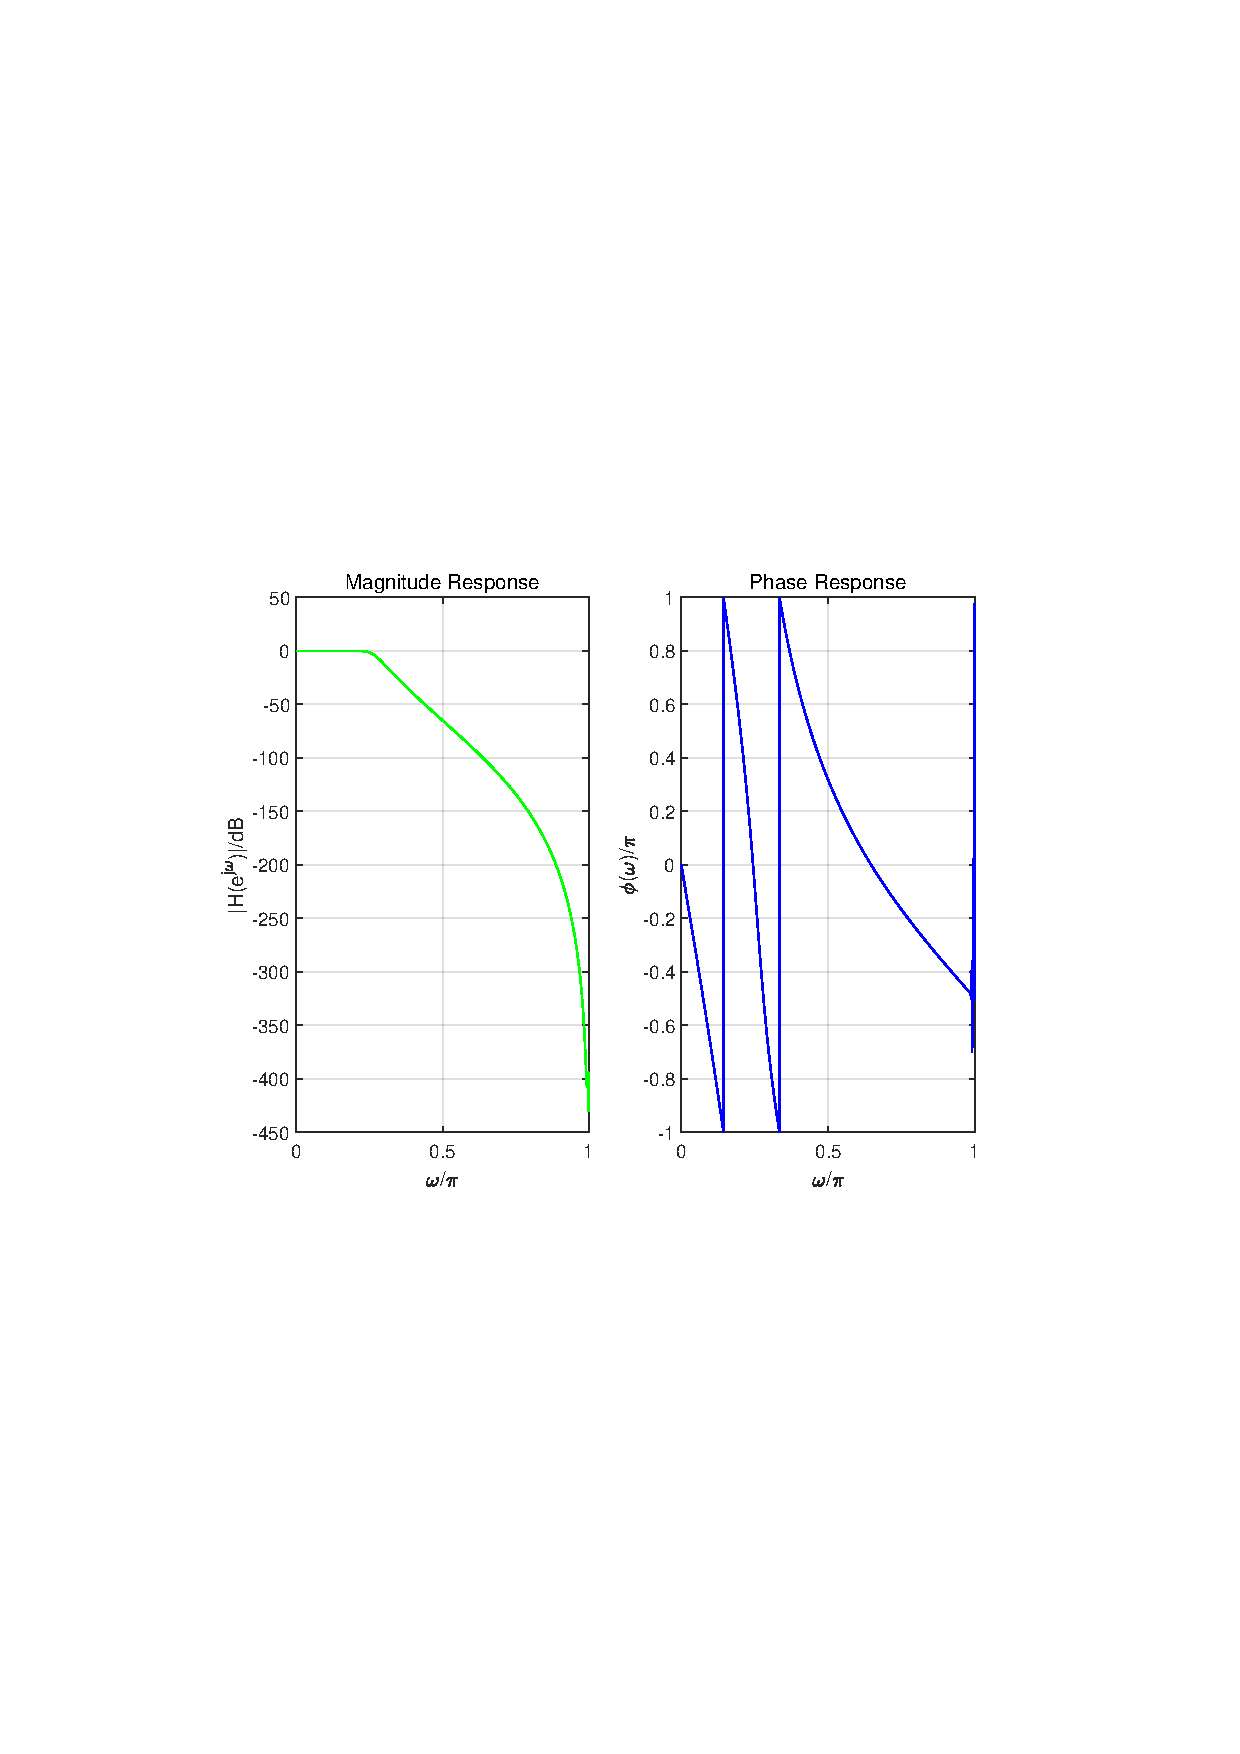
\includegraphics[width=0.7\textwidth]{figure/LPBF.pdf}
	\caption{数字低通滤波器幅频特性和相频特性曲线} \label{fig:LPBF}
\end{figure}

\subsection{问题 4}

求解滤波器参数得到阶数 $N=9$,3dB 截止频率$Wc=0.2615$,滤波器系统函数的分子、分母多项式系数向量如下:
%
\begin{align}
B &= 0.0000\ 0.0004\ 0.0017\ 0.0041\ 0.0061\ 0.0061\ 0.0041\ 0.0017\ 0.0004\ 0.0000 \\
A &= 1.0000\ -4.2785\ 8.8461\ -11.2842\ 9.6717\ -5.7301\ 2.3339\ -0.6276\ 0.1008\ -0.0073
\end{align}

根据 Matlab 官网函数说明,得到的系统函数形式如下:
%
\begin{equation}
H(z)=\frac{B(z)}{A(z)}=\frac{b(1)+b(2)z^{-1}+\cdots+b(n+1)z^{-n}}{a(1)+a(2)z^{-1}+\cdots+a(n+1)z^{-n}}
\end{equation}

数字低通滤波器 $H(z)$ 结构信号流图如图 \ref{fig:signalflow} 所示。

\begin{figure}[htbp]
	\centering
	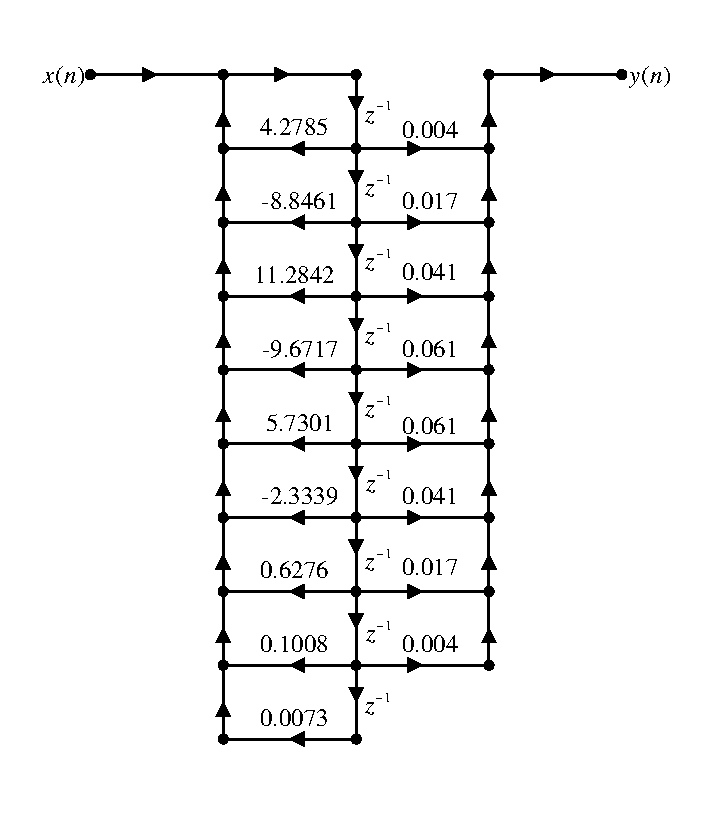
\includegraphics[width=0.7\textwidth]{figure/signalflow.pdf}
	\caption{数字低通滤波器 $H(z)$ 结构信号流图} \label{fig:signalflow}
\end{figure}

\subsection{问题 5}

将合成信号 $x(n)$ 输入数字滤波器 $H(z)$,得到输出响应 $y(n)$,其时域波形和频谱图如图 \ref{fig:yn} 所示。可见,经过数字滤波器 $H(z)$ 滤波后,大于截止频率的分量被滤除,满足低通滤波的要求。

\begin{figure}[htbp]
	\centering
	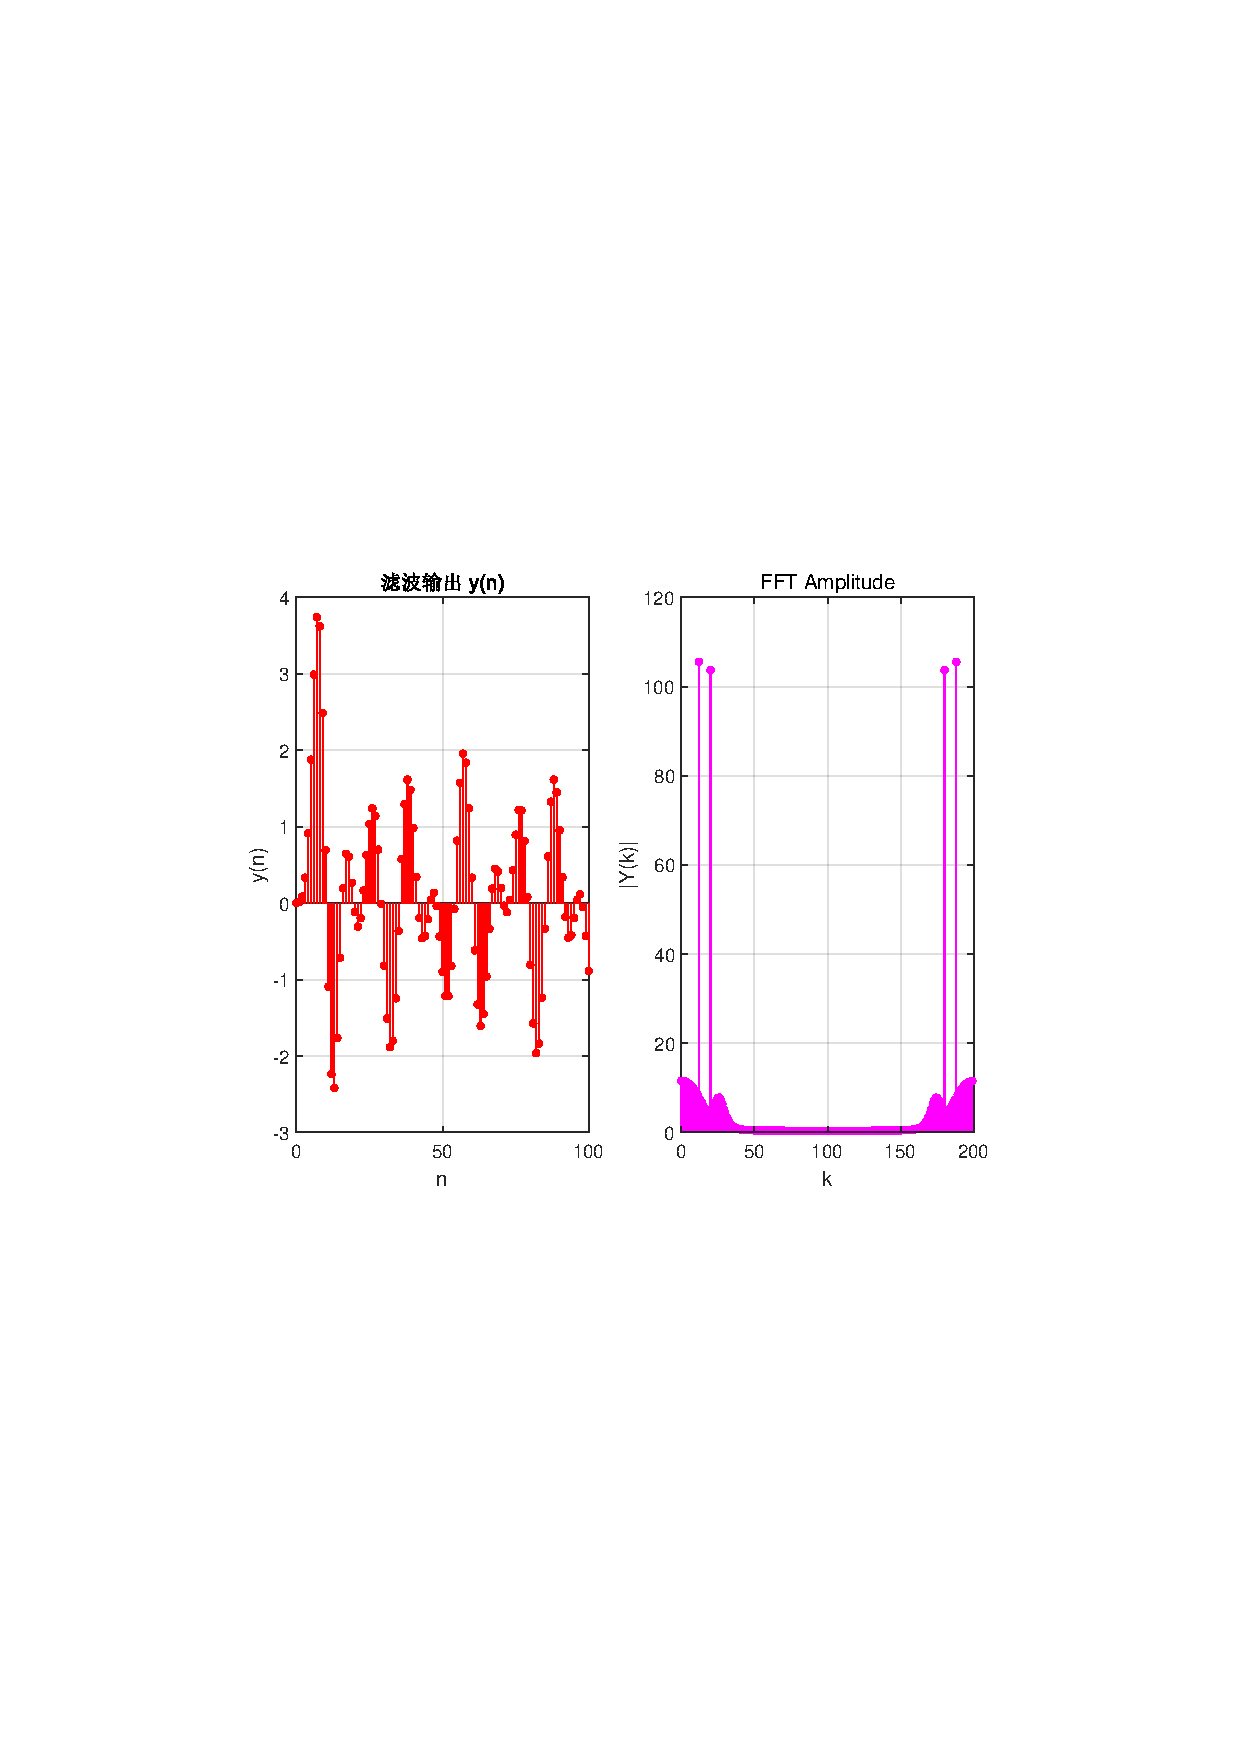
\includegraphics[width=0.7\textwidth]{figure/yn.pdf}
	\caption{滤波器输出响应 $y(n)$ 的时域波形和频谱图} \label{fig:yn}
\end{figure}

\section{总结}

在本文中,我们针对数字信号处理课程设计要求,用 Visio 绘制了实验流程图如图 \ref{fig:workflow} 所示,针对实验流程用 Matlab 和 Python 两种语言进行编程实验与分析,绘制了 $sa_1(t)$、$sa_2(t)$、$xa(t)$ 三个模拟信号的时域波形和频谱图以及 $s_1(n)$、$s_2(n)$、$x(n)$ 三个离散信号的时域波形和频谱图,通过观测频谱特征,我们选择巴特沃斯数字低通滤波器进行滤波,并绘制滤波器的幅频特性和相频特性曲线,其指标满足设计要求,将 $x(n)$ 输入滤波器获得 $y(n)$,并绘制其时域波形和频谱图,最后结果符合我们的预期。本文设计的有用信号和干扰信号较为简单,但实际中的信号却都较为复杂,工业上设计滤波器流程较为复杂,需要更加深入学习相关知识并灵活运用。通过这次实验我们夯实了相关基础知识,能够较好地使用 Matlab 和 Python 进行信号处理,对 \LaTeX 和 Visio 软件使用也更加熟练。


% % 参考文献,此处以 MLA 引用格式为例

% \begin{thebibliography}{9}
%     \bibitem{1} Dijkstra, Edsger Wybe. "A Note on Two Problems in Connexion With Graphs." \emph{Numerische Mathematik} 1(1959):269-271.
% \end{thebibliography}


% \includepdf[pages={1,2}]{Memo.pdf} 
% 可以直接导入pdf页面
\newpage
\begin{appendices}  % 附录环境
\section{Matlab 代码}

\begin{lstlisting}[language=Matlab]
% 问题 1
N = 2000; L = 2; k = 0:N-1;
dt = L / N; t = k * dt; f = k / L;

f1 = 10; f2 = 6; f3 = 36; f4 = 25;
sa1 = cos(2*pi*f1*t)+cos(2*pi*f2*t);
sa2 = 10*cos(2*pi*f3*t)+10*cos(2*pi*f4*t);
xa = sa1 + sa2;
F1 = fft(sa1,N);
F2 = fft(sa2,N);
F3 = fft(xa,N);

figure(1);
subplot(1,2,1)
plot(t,sa1,'b','LineWidth',0.8); grid on;
xlabel('t/s'); ylabel('sa_1(t)');
xlim([0 1]); title('有用信号');

subplot(1,2,2)
plot(f,0.5*abs(F1)/max(abs(F1)),'g','LineWidth',0.8); grid on;
xlabel('f/Hz'); ylabel('F(j2\pif)');
axis([0 40 0 1]); title('频谱图');

figure(2);
subplot(1,2,1)
plot(t,sa2,'b','LineWidth',0.8); grid on;
xlabel('t/s'); ylabel('sa_2(t)');
xlim([0 1]); title('干扰信号');

subplot(1,2,2)
plot(f,5*abs(F2)/max(abs(F2)),'g','LineWidth',0.8); grid on;
xlabel('f/Hz'); ylabel('F(j2\pif)');
axis([0 40 0 10]); title('频谱图');

figure(3);
subplot(1,2,1)
plot(t,xa,'b','LineWidth',0.8); grid on;
xlabel('t/s'); ylabel('xa(t)');
xlim([0 1]); title('合成信号');

subplot(1,2,2)
plot(f,5*abs(F3)/max(abs(F3)),'g','LineWidth',0.8); grid on;
xlabel('f/Hz'); ylabel('F(j2\pif)');
axis([0 40 0 10]); title('频谱图');

% 问题 2
Fs = 100; Ts = 1 / Fs; n = 0:199;
tn = n * Ts;
sn1 = cos(2*pi*f1*tn)+cos(2*pi*f2*tn);
sn2 = 10*cos(2*pi*f3*tn)+10*cos(2*pi*f4*tn);
xn = sn1 + sn2;
Fn1 = fft(sn1);
Fn2 = fft(sn2);
Fn3 = fft(xn);

figure(4);
subplot(1,2,1)
stem(n,sn1,'r','filled','LineWidth',0.6,'MarkerSize',3); grid on;
xlabel('n'); ylabel('s_1(n)');
xlim([0 100]); title('离散有用信号');

subplot(1,2,2)
stem(abs(Fn1),'m','filled','LineWidth',0.6,'MarkerSize',3); grid on;
xlabel('k'); ylabel('|S_1(k)|');
title('FFT Amplitude')

figure(5);
subplot(1,2,1)
stem(n,sn2,'r','filled','LineWidth',0.6,'MarkerSize',3); grid on;
xlabel('n'); ylabel('s_2(n)');
xlim([0 100]); title('离散干扰信号');

subplot(1,2,2)
stem(abs(Fn2),'m','filled','LineWidth',0.6,'MarkerSize',3); grid on;
xlabel('k'); ylabel('|S_2(k)|');
title('FFT Amplitude')

figure(6);
subplot(1,2,1)
stem(n,xn,'r','filled','LineWidth',0.6,'MarkerSize',3); grid on;
xlabel('n'); ylabel('x(n)');
xlim([0 100]); title('离散合成信号');

subplot(1,2,2)
stem(abs(Fn3),'m','filled','LineWidth',0.6,'MarkerSize',3); grid on;
xlabel('k'); ylabel('|X(k)|');
title('FFT Amplitude')

% 问题 3
fp=12; fs=20;
Wp=2*fp/Fs; Ws=2*fs/Fs; Rp=1; Rs=40;
[N,Wc] = buttord(Wp,Ws,Rp,Rs)
[B,A] = butter(N,Wc)
[H,w] = freqz(B,A,1000);

figure(7);
subplot(1,2,1);
plot(w/pi, 20*log10(abs(H)),'g','LineWidth',0.8); grid on;
xlabel('\omega/\pi'); ylabel('|H(e^j^\omega)|/dB');
title('Magnitude Response');

subplot(1,2,2);
plot(w/pi, angle(H)/pi,'b','LineWidth',0.8); grid on;
xlabel('\omega/\pi'); ylabel('\phi(\omega)/\pi');
title('Phase Response');

% 问题 5
yn = filter(B,A,xn);
Yk = fft(yn);

n = 0:length(yn)-1;
figure(8);
subplot(1,2,1)
stem(n,yn,'r','filled','LineWidth',0.6,'MarkerSize',3); grid on;
% plot(n,yn,'b','LineWidth',1); hold on; grid on;
xlabel('n'); ylabel('y(n)');
xlim([0 100]); title('滤波输出 y(n)');

subplot(1,2,2)
stem(n,abs(Yk),'m','filled','LineWidth',0.6,'MarkerSize',3); grid on;
xlabel('k'); ylabel('|Y(k)|');
title('FFT Amplitude')
\end{lstlisting}

\includepdfset{pagecommand={\thispagestyle{fancy}}} 
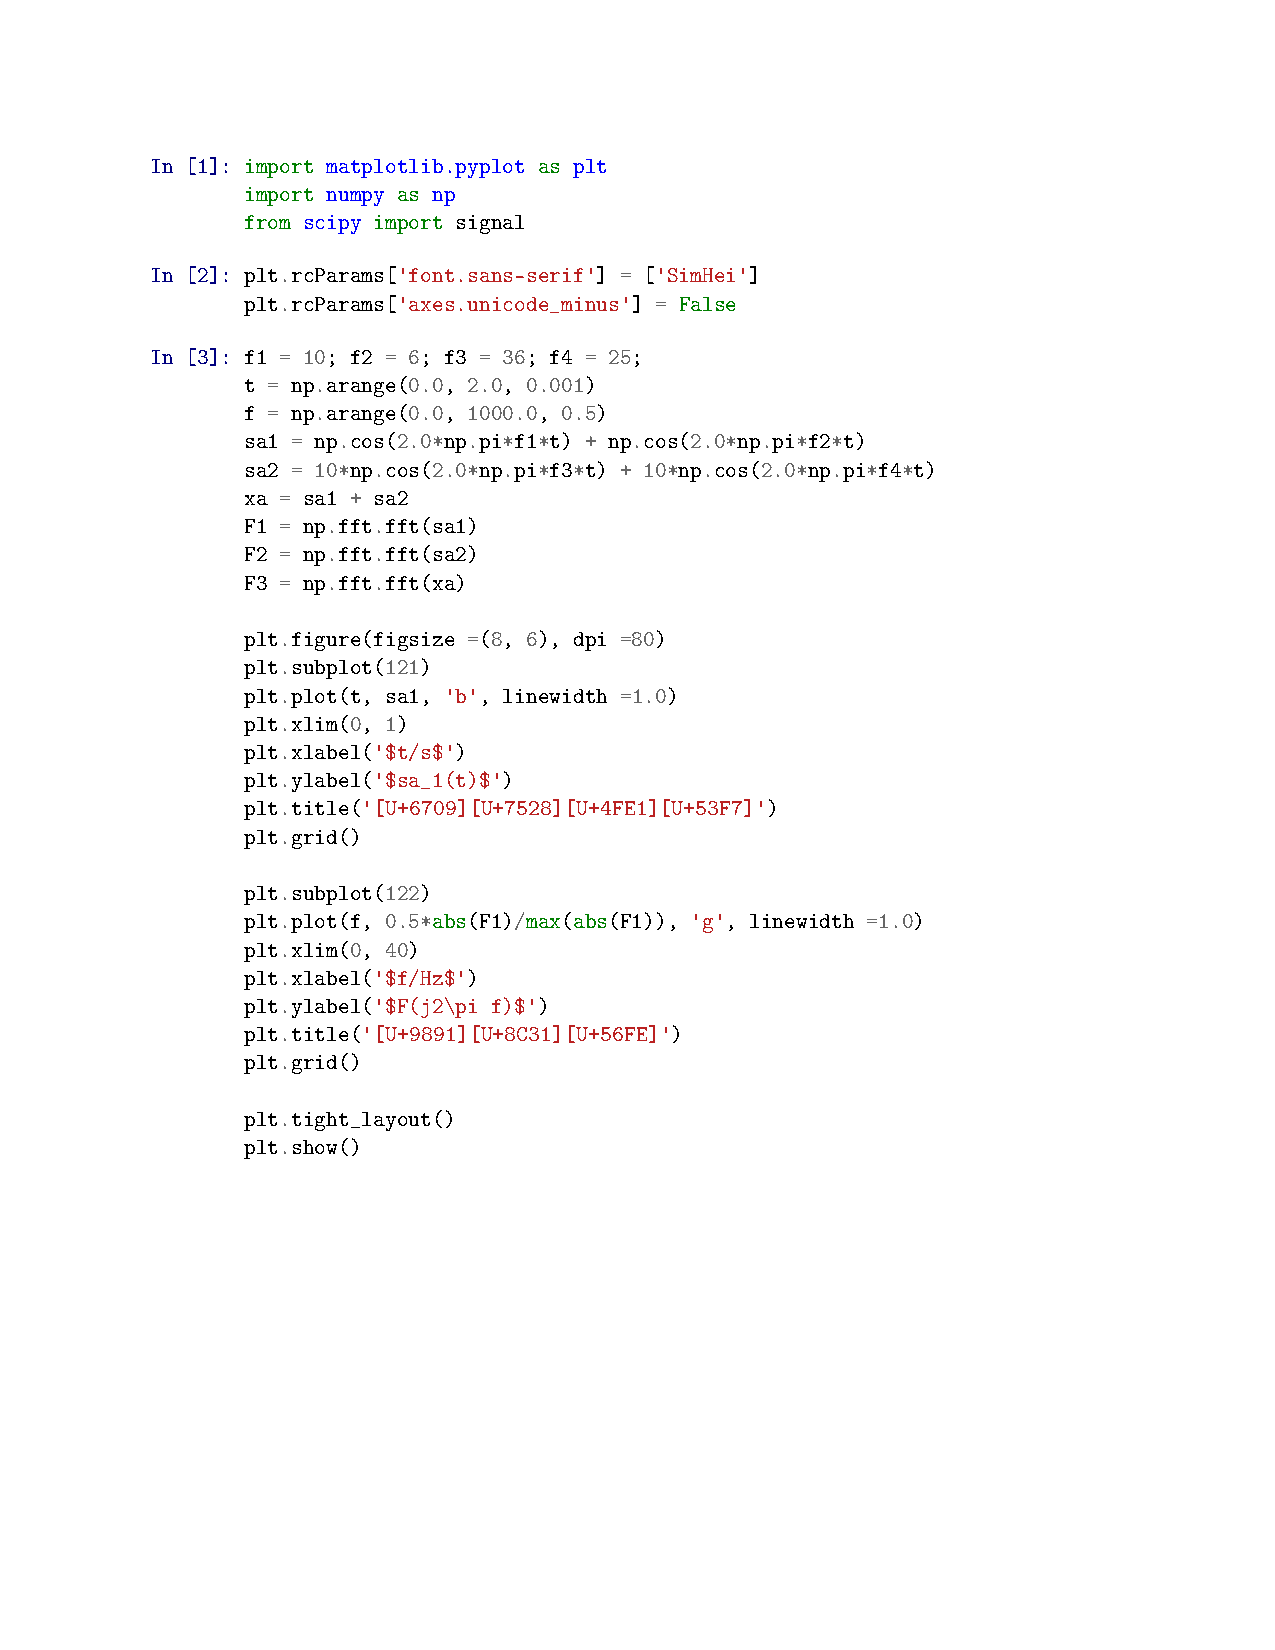
\includepdf[addtotoc={1, section, 2, Python 代码,pythoncode},pages=1-9,offset=0cm 0cm]{JupyterNotebook.pdf} 

\end{appendices}

\end{document}  % 结束